\documentclass[tikz,14pt,fleqn]{article}


\usepackage[utf8]{inputenc}
\usepackage[margin=1in]{geometry}
\usepackage[titletoc,title]{appendix}
\usepackage{latexsym}
\usepackage{amssymb}
\usepackage{gensymb}
\usepackage{amsmath}
\usepackage{amsfonts}
\usepackage[dvipsnames]{xcolor}
\usepackage{multicol}
\usepackage{graphicx}
\usepackage{fancyhdr}
\usepackage[linguistics]{forest}
\usepackage{colortbl}
\usepackage{pdfpages}
\usepackage{wrapfig}
\usepackage{cleveref}


% to fixme
\usepackage{xcolor} 
\definecolor{FIXMECOLOR}{rgb}{1,0,0}
\newcommand{\FIXME}[1]{{\color{FIXMECOLOR}{\textbf{FIXME: #1}}}} 

% to simplify math 
\newcommand{\pvec}[3]{
   \ensuremath{
   \begin{pmatrix}
       #1 \\
       #2 \\
       #3
   \end{pmatrix}
}}

\newcommand{\bvec}[3]{
   \ensuremath{
   \begin{bmatrix}
       #1 \\
       #2 \\
       #3
   \end{bmatrix}
}}

\newcommand{\bmat}[9]{
   \ensuremath{
   \begin{bmatrix}
       #1 & #2 & #3 \\
       #4 & #5 & #6 \\
       #7 & #8 & #9
   \end{bmatrix}
}}

\newcommand{\dotproduct}[2]{\ensuremath{\left< #1, #2 \right>}}

%% For plotting
\usepackage{pgfplots}
\pgfplotsset{width=10cm,compat=1.9}
\usepgfplotslibrary{external}
\tikzexternalize
%%
\usepackage{dirtree}
\usepackage{subcaption}
\usepackage{xifthen}% provides \isempty test
\usepackage{glossaries}

\captionsetup[subfigure]{labelformat=empty}
\definecolor{color1}{HTML}{0B0C10}
\definecolor{color2}{HTML}{1F2833}
\definecolor{color3}{HTML}{C5C6C7}
\definecolor{color4}{HTML}{66FCF1}
\definecolor{color5}{HTML}{45A29E}

\pagestyle{fancy}
\fancyhf{}
%%%%%%%%%%%%%%%%%%%%%%%%%%%%
%% VARIABLES
\newcommand\namesurname{Albert Cerfeda\\Alessandro Gobbetti}
\newcommand\assignment{Assignment 4}

\newcommand\subject{Computer Graphics}
\newcommand\documentdate{18.10.2022}

% Title content
%%%%%%%%%%%%%%%%%%%%%%%%%%%%
\rhead{\assignment}
\lhead{\namesurname}
%%%%%%%%%%%%%%%%%%%%%%%%%%%%
\rfoot{Page \thepage}
\setlength{\parindent}{0pt}

\newcommand\xdownarrow[1][2ex]{%
   \mathrel{\rotatebox{90}{$\xleftarrow{\rule{#1}{0pt}}$}}
}

\begin{document}

\begin{titlepage}
   \begin{center}
       \vspace*{1cm}

       \textbf{\Large{Homework Assignment}}

       \vspace{0.5cm}
        \textbf{\subject}\\[5mm]
       \assignment
        
            
       \vspace{1.8cm}

        \namesurname
       \tableofcontents

       \vspace*{\fill}
     
       \includegraphics[width=0.4\textwidth]{fig/logo.png}
       
        \documentdate \\
        Università della Svizzera italiana\\
        Faculty of Informatics\\
        Switzerland\\

   \end{center}
\end{titlepage}



\section{Exercise 1}
\subsection{Task 1}
\[
R_{90} = 
\begin{bmatrix}
cos(\alpha) & -sin(\alpha) & 0\\
sin(\alpha) & cos(\alpha) & 0\\
0 & 0 & 1
\end{bmatrix} = 
\begin{bmatrix}
cos(90) & -sin(90) & 0\\
sin(90) & cos(90) & 0\\
0 & 0 & 1
\end{bmatrix} =
\begin{bmatrix}
0 & -1 & 0\\
1 & 0 & 0\\
0 & 0 & 1
\end{bmatrix}
\]

% translation matrix T
\[
T =
\begin{bmatrix}
1 & 0 & 1\\
0 & 1 & -2\\
0 & 0 & 1
\end{bmatrix}
\]


\subsection{Task 2}
Represent $p_1 = (1, 1)^T$ and $p = (1.5, 2.5)^T$ and $u = p - p_1 = (0.5, 1.5)^T$ in homogeneous coordinates:
\[
p_1 = (1,1,1)^T, \quad p = (1.5,2.5,1)^T, \quad u = (0.5,1.5,0)^T
\]
Rotate the points and the vector:
\[
R_{90} \cdot p_1=
\begin{bmatrix}
0 & -1 & 0\\
1 & 0 & 0\\
0 & 0 & 1
\end{bmatrix}
\begin{bmatrix}
1\\
1\\
1
\end{bmatrix}=
\begin{bmatrix}
-1\\
1\\
1
\end{bmatrix}
\quad p_{1_{90}} = (-1,1)^T
\]

\[
R_{90} \cdot p=
\begin{bmatrix}
0 & -1 & 0\\
1 & 0 & 0\\
0 & 0 & 1
\end{bmatrix}
\begin{bmatrix}
1.5\\
2.5\\
1
\end{bmatrix}=
\begin{bmatrix}
-2.5\\
1.5\\
1
\end{bmatrix}
\quad p_{90} = (-2.5, 1.5)^T
\]

\[
R_{90} \cdot u=
\begin{bmatrix}
0 & -1 & 0\\
1 & 0 & 0\\
0 & 0 & 1
\end{bmatrix}
\begin{bmatrix}
0.5\\
1.5\\
0
\end{bmatrix}=
\begin{bmatrix}
-1.5\\
0.5\\
0
\end{bmatrix}
\quad u_{90} = (-1.5, 0.5)^T
\]

Translate the rotated points and vector:
\[
T \cdot p_{1_{90}}=
\begin{bmatrix}
1 & 0 & 1\\
0 & 1 & -2\\
0 & 0 & 1
\end{bmatrix}
\begin{bmatrix}
-1\\
1\\
1
\end{bmatrix}=
\begin{bmatrix}
0\\
-1\\
1
\end{bmatrix}
\quad p'_1 = (0,-1)^T
\]

\[
T \cdot p_{90}=
\begin{bmatrix}
1 & 0 & 1\\
0 & 1 & -2\\
0 & 0 & 1
\end{bmatrix}
\begin{bmatrix}
-2.5\\
1.5\\
1
\end{bmatrix}=
\begin{bmatrix}
-1.5\\
-0.5\\
1
\end{bmatrix}
\quad p' = (-1.5,-0.5)^T
\]

\[
T \cdot u_{90}=
\begin{bmatrix}
1 & 0 & 1\\
0 & 1 & -2\\
0 & 0 & 1
\end{bmatrix}
\begin{bmatrix}
-1.5\\
0.5\\
0
\end{bmatrix}=
\begin{bmatrix}
-1.5\\
0.5\\
0
\end{bmatrix}
\quad u' = (-1.5,0.5)^T
\]

Verify that $u' = p' - p'$:
\[
   p' - p'_1
   =
   \begin{bmatrix}
   -1.5\\
   -0.5\\
   \end{bmatrix}
   -
   \begin{bmatrix}
   0\\
   -1\\
   \end{bmatrix}
   =
   \begin{bmatrix}
   -1.5\\
   0.5\\
   \end{bmatrix}
   =
   u'
\]

Since $u$ is a vector, it is not affected by the translation. Thus, $u' = u$.

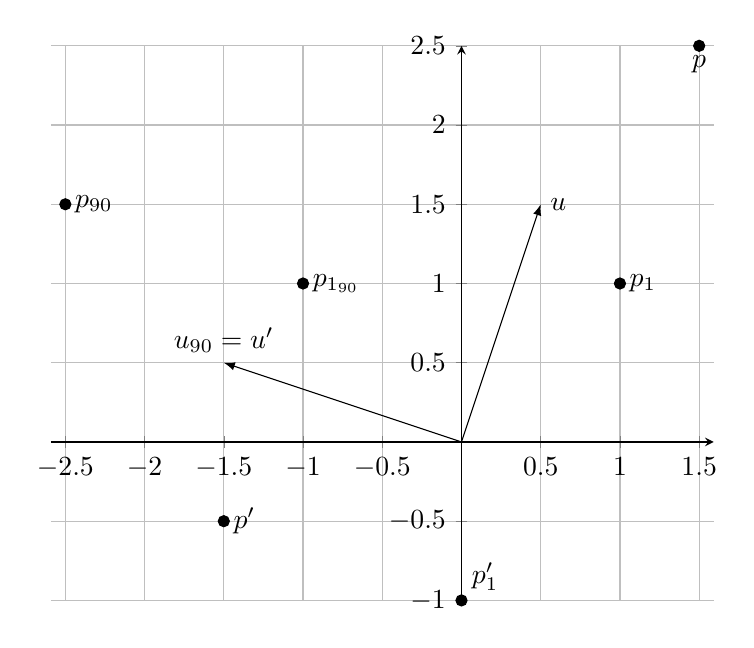
\begin{tikzpicture}
   \begin{axis}[axis lines=middle,axis equal,grid=both]
      \addplot[mark=*,only marks] coordinates {(1,1)} node[right] {$p_1$};
      \addplot[mark=*,only marks] coordinates {(1.5,2.5)} node[below] {$p$};
      \addplot[mark=,->,>=latex] coordinates {(0,0) (0.5,1.5)} node[right] {$u$};
      
      \addplot[mark=*,only marks] coordinates {(-1,1)} node[right] {$p_{1_{90}}$};
      \addplot[mark=*,only marks] coordinates {(-2.5,1.5)} node[right] {$p_{90}$};
      
      \addplot[mark=*,only marks] coordinates {(0,-1)} node[above, xshift=0.3cm] {$p'_1$};
      \addplot[mark=*,only marks] coordinates {(-1.5,-0.5)} node[right] {$p'$};
      
      \addplot[mark=,->,>=latex] coordinates {(0,0) (-1.5,0.5)} node[above] {$u_{90} = u'$};
   \end{axis}
\end{tikzpicture}


\subsection{Task 3}

Scaling matrix:
\[
S = \begin{bmatrix}
2 & 0 & 0\\
0 & 2 & 0\\
0 & 0 & 1
\end{bmatrix}
\]

\[
S \cdot p'_1= 
\begin{bmatrix}
2 & 0 & 0\\
0 & 2 & 0\\
0 & 0 & 1
\end{bmatrix}
\begin{bmatrix}
0\\
-1\\
1
\end{bmatrix}=
\begin{bmatrix}
0\\
-2\\
1
\end{bmatrix}
\quad p''_1 = (0,-2)^T
\]

\[
S \cdot p'=
\begin{bmatrix}
2 & 0 & 0\\
0 & 2 & 0\\
0 & 0 & 1
\end{bmatrix}
\begin{bmatrix}
-1.5\\
-0.5\\
1
\end{bmatrix}=
\begin{bmatrix}
-3\\
-1\\
1
\end{bmatrix}
\quad p'' = (-3,-1)^T
\]

\[
S \cdot u'=
\begin{bmatrix}
2 & 0 & 0\\
0 & 2 & 0\\
0 & 0 & 1
\end{bmatrix}
\begin{bmatrix}
-1.5\\
0.5\\
0
\end{bmatrix}=
\begin{bmatrix}
-3\\
1\\
0
\end{bmatrix}
\quad u'' = (-3,1)^T
\]

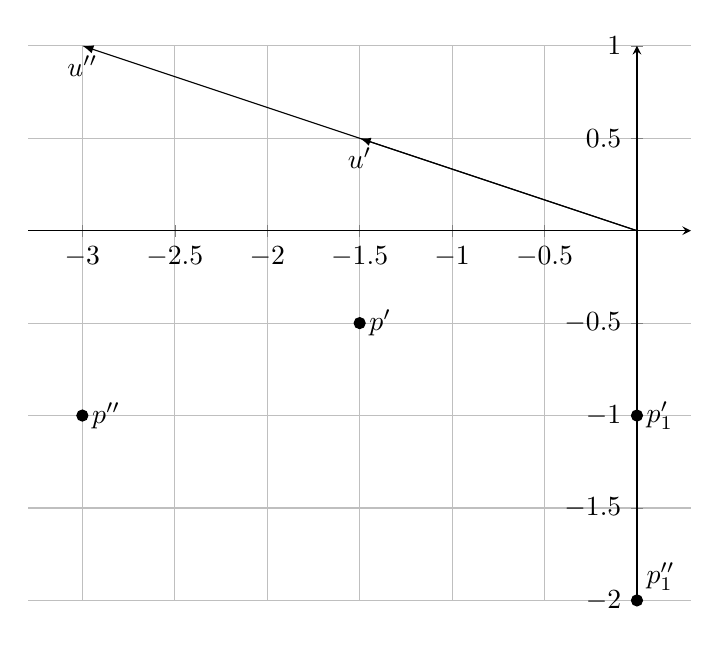
\begin{tikzpicture}
   \begin{axis}[axis lines=middle,axis equal,grid=both]
      \addplot[mark=*,only marks] coordinates {(0,-1)} node[right] {$p'_1$};
      \addplot[mark=*,only marks] coordinates {(-1.5,-0.5)} node[right] {$p'$};
      \addplot[mark=,->,>=latex] coordinates {(0,0) (-1.5,0.5)} node[below] {$u'$};
      
      \addplot[mark=*,only marks] coordinates {(0,-2)} node[above, xshift=0.3cm] {$p''_1$};
      \addplot[mark=*,only marks] coordinates {(-3,-1)} node[right] {$p''$};
      \addplot[mark=,->,>=latex] coordinates {(0,0) (-3,1)} node[below] {$u''$};

   \end{axis}
\end{tikzpicture}



\subsection{Task 4}

Compute inverse matrix of S:
\[
S^{-1} = \begin{bmatrix}
\frac{1}{2} & 0 & 0\\
0 & \frac{1}{2} & 0\\
0 & 0 & 1
\end{bmatrix}
\]



\section{Exercise 2}

% Consider a triangle made of three points p1 = (6, 0, 4), p2 = (2, 0, 0), and p3 = (2, 4, 4). 
% Verify whether point p = (4, 1, 3) belongs to the interior of the triangle

\[
   p_1 = (6, 0, 4),\quad p_2 = (2, 0, 0),\quad p_3 = (2, 4, 4)
\]
\[
   p = (4, 1, 3)
\]

Normal of triangle [$p_1$, $p_2$, $p_3$]:
\[
   n = (p_2 - p_1) \times (p_3 - p_1) = 
   \left(
   \pvec{2}{0}{0} - \pvec{6}{0}{4}
   \right)
   \times
   \left(
   \pvec{2}{4}{4} - \pvec{6}{0}{4}
   \right) =
   \pvec{-4}{0}{-4}
   \times
   \pvec{-4}{4}{0}
   =
   \pvec{16}{16}{-16}
\]


Normals of the sub-triangles:
\[
   n_1 = (p_3 - p) \times (p_1 - p) =
   \left(
   \pvec{2}{4}{4} - \pvec{4}{1}{3}
   \right)
   \times
   \left(
   \pvec{6}{0}{4} - \pvec{4}{1}{3}
   \right) =
   \pvec{-2}{3}{1}
   \times
   \pvec{2}{-1}{1}
   =
   \pvec{4}{4}{-4}
\]



\[
   n_2 = (p_1 - p) \times (p_2 - p) =
   \left(
   \pvec{6}{0}{4} - \pvec{4}{1}{3}
   \right)
   \times
   \left(
   \pvec{2}{0}{0} - \pvec{4}{1}{3}
   \right) =
   \pvec{2}{-1}{1}
   \times
   \pvec{-2}{-1}{-3}
   =
   \pvec{4}{4}{-4}
\]


\[
  n_3 = (p_2 - p) \times (p_3 - p) =
   \left(
   \pvec{2}{0}{0} - \pvec{4}{1}{3}
   \right)
   \times 
   \left(
   \pvec{2}{4}{4} - \pvec{4}{1}{3}
   \right) =
   \pvec{-2}{-1}{-3}
   \times
   \pvec{-2}{3}{1}
   =
   \pvec{8}{8}{-8}
\]


Then compute the signs between the obtained sub-triangles normals with the normal of the triangle:
\[
   sign(\dotproduct{n_1}{n}) = 
   sign
   \left(
   \dotproduct{\pvec{4}{4}{-4}}{\pvec{16}{16}{-16}}
   \right) = 
   sign(64 + 64 + 64 ) = sign(192) = +1
\]

\[
   sign(\dotproduct{n_2}{n}) = 
   sign
   \left(
   \dotproduct{\pvec{4}{4}{-4}}{\pvec{16}{16}{-16}}
   \right) = 
   sign(64 +64 +64 ) = sign(192) = +1
\]

\[
   sign(\dotproduct{n_3}{n}) = 
   sign
   \left(
   \dotproduct{\pvec{8}{8}{-8}}{\pvec{16}{16}{-16}}
   \right) = 
   sign(128 +128 +128) = sign(384) = +1
\]

Since every sign is positive, the point is inside the triangle.



\section{Exercise 3}

\section{Exercise 4}

\section{Bonus exercise 5}



\end{document}